\documentclass{article}
\usepackage[UTF8]{ctex}
\usepackage{geometry}
\usepackage{natbib}
\geometry{left=3.18cm,right=3.18cm,top=2.54cm,bottom=2.54cm}
\usepackage{graphicx}
\pagestyle{plain}	
\usepackage{setspace}
\usepackage{caption2}
\usepackage{datetime} %日期
\renewcommand{\today}{\number\year 年 \number\month 月 \number\day 日}
\renewcommand{\captionlabelfont}{\small}
\renewcommand{\captionfont}{\small}
\begin{document}

\begin{figure}
    \centering
    
\includegraphics[width=8cm]{upc.png}

    \label{figupc}
\end{figure}

	\begin{center}
		\quad \\
		\quad \\
		\heiti \fontsize{45}{17} \quad \quad \quad 
		\vskip 1.5cm
		\heiti \zihao{2} 《计算科学导论》课程总结报告
	\end{center}
	\vskip 2.0cm
		
	\begin{quotation}
% 	\begin{center}
		\doublespacing
		
        \zihao{4}\par\setlength\parindent{7em}
		\quad 

		学生姓名:\underline{\qquad  黄淳 \qquad \qquad}

		学\hspace{0.61cm} 号:\underline{\qquad 1907010108\qquad}
		
		专业班级:\underline{\qquad 计科1901 \qquad  }
		
        学\hspace{0.61cm} 院:\underline{计算机科学与技术学院}
% 	\end{center}
		\vskip 2cm
		\centering
		\begin{table}[h]
            \centering 
            \zihao{4}
            \begin{tabular}{|c|c|c|c|c|c|c|}
            % 这里的rl 与表格对应可以看到,姓名是r,右对齐的;学号是l,左对齐的;若想居中,使用c关键字。
                \hline
                课程认识 & 问题思 考 & 格式规范  & IT工具  & Latex附加  & 总分 & 评阅教师 \\
                30\% & 30\% & 20\% & 20\% & 10\% &  &  \\
                \hline
                 & & & & & &\\
                & & & & & &\\
                \hline
            \end{tabular}
        \end{table}
		\vskip 2cm
		\today
	\end{quotation}

\thispagestyle{empty}
\newpage
\setcounter{page}{1}
% 在这之前是封面,在这之后是正文
\section{引言}
一个学期的计算科学导论课程已经结束了。在孙运雷老师的指引下,我们完成了计算科学导论的学期。从一开始的一头雾水,到现在了解了这门课程的大体框架,认识了许许多多的新知识。也获得了新的学习方法和新的心得体会。孙老师注重知识体系架构的构建,注重引导我们思考,注重培养学生的自主学习能力和团队协作能力。此外,孙老师更加注重培养学生的社会责任感,教导学生从事对人民,对国家有益处的事业。若科研,则为中国理论计算机事业发光发热;若要工作,则要恪守本心,在如华为一样有社会责任感,传播社会主义核心价值观的优秀企业尽一份力。切不能为眼前利益忘记本心,要做爱国爱党的好青年。\par
在孙老师的教导下,我在这门课中受益良多,不仅从宏观上了解了计算科学这门学科的发展史、现状和与其他学科的联系等内容,也感受到了孙老师所讲的“导论”作为一门学科的指导与方法论的美丽与功用。

\section{对计算科学导论这门课程的认识、体会}
不同于大多数《计算科学导论》教材在内容上编成计算机科学与技术本科专业课程教学内容简洁压缩版的情况,赵致琢先生所编纂的《计算科学导论》首先从本科一年级学生学习中普遍关心的问题出发,就学科特点、学科形态、历史渊源、发展变化、典型方法、学习知识组织结构和分类体系、各年级课程的终点,以及如何认识计算科学,学好计算科学等问题从科学哲学和高级科普的角度去回答我们的疑问。\par
与此同时,导论的内容与后续课程的衔接也有科学的论证,课上所学计算科学导论的知识,在我尚未具有学习后续课程必要的基础知识的情况下,没有在短暂的课程中为我们灌输这些知识,而是为我们以后的专业课学习指明了框架与方向。\par
可以说,孙老师开设的这门计算科学导论,的的确确达到了教材作者与孙老师心目中“高级科普”、“科学哲学”、“学科方法论”的目的,于我本身,这样一门导论课程使我受益匪浅。

\subsection{科学哲学与学科方法论}
在第一章的引论中,赵致琢先生由浅入深,层层深入地为我们介绍了了“计算科学一词的来历”、“科学哲学与学科方法论”、“一般的科学思想方法”等内容,还为如我一般计算机初学者提供了宝贵的意见。\par
在教材正文一开始,同样也是孙老师为我们讲授计算科学导论的第一节课,我们就接触了“计算科学一词的来历”。短短几页文字,短短半堂课,便为我等懵懂而又无知的一年级新生揭开了“我从哪里来”这一宏大问题的答案。作为一名计算机科学与技术专业的学生,理应知道自己的学科,自己所主修的专业课如何在历史的洪流中,在时代的浪潮下汇聚成为一门完整的、成体系的学科,理应思考并探索“我从哪里来”这个宏大的问题。若不然,我们的思想将会缺乏根基,直接影响到我们在本科阶段乃至以后整个人生的规划与发展。\par
而紧随其后对科学哲学与学科方法论的简介,则是简单明了的向我们点出了这门课程的意义与重要性。从自然科学依附于哲学母体,到17世纪初近代自然科学开始形成,同时自然科学逐渐分离出来,再到数学、物理学等诸多自然科学在发展中因危机而发生了剧烈的变革,从而迫使科学家们反思而提出一系列自然科学的哲学问题,如科学的认识论基础和逻辑基础问题。在此过程中哲学与自然科学一直相伴相生,如影随形。科学哲学的重要性不言而喻。而作为科学哲学研究中最重要的研究内容之一——科学方法论,和某一具体学科的结合——学科方法论,更是可以指引每一个深耕于其中的科学家,为其提供灵感与方向。\par
而这门课所介绍的计算科学初学者的正确选择更让我感动,在这一堂课中,我不仅明白了何为优秀的计算机科学与技术专业人才,更了解到了在现阶段我对整个学科还缺乏深入、全面了解的情况下该如何去思考,如何去学习。

\subsection{计算的数学理论}
随着之后课程学习的不断深入,书中描绘的计算科学的内容与结构,计算科学的美妙世界在我脑海中也越发清晰。\par
其中第三章中介绍的“计算的数学理论”,也就是计算理论、高等逻辑、形式语言与自动机和形式语义学等内容更是引发了我的思考,使我对这些内容产生了浓厚了兴趣。\par
不管是赵先生所编纂的教材,还是孙老师精心准备的课堂,对这些本身深奥而晦涩,复杂且高深的内容,并不是丢出一串接一串的定义、定理、引理、证明,而是用深入浅出且生动形象的例子,令我大开眼界,如醍醐灌顶,受益匪浅。

\subsection{从最小确定性有限状态自动机到后缀自动机}
计算科学导论课上对形式语言与自动机的描述,引发了我对自动机理论的兴趣,于是阅读了期刊论文\emph{Introduction to Automata Theory, Languages, and Computation}\cite{ref1}与\emph{Finite automata}\cite{ref2},了解了自动机理论与有限状态自动机的基本知识。\par
确定性有限状态自动机(Deterministic Finite Automation, DFA)可以被用来解决匹配问题,但是状态和转移的数量会极大地影响一个DFA的运行效率与在计算机中所需的存储空间,例如:\par
给定一个长度为$n$的字符串,试构造一个确定性有限状态自动机,使得这个DFA可以识别该字符串的任意后缀。\par
最朴素的做法是将$n$个后缀依次插入一棵Trie树中,然而这个做法的时空复杂度都是$O(n^2)$的,运行效率低下,所占内存巨大。\par
\emph{Introduction to the Theory of Computation}\cite{ref3}给出了等价类自动机、最小等价确定性有限状态自动机的定义,以及对于任意的确定性有限状态自动机,其最小等价自动机唯一的证明,这使得我们拥有了强有力的理论基础来简化上述朴素做法中的Trie树。\par
根据\emph{The smallest automation recognizing the subwords of a text}\cite{ref4},这个简化的结果就是后缀自动机,现如今解决子串匹配及后缀识别效率最高最有力的数据结构。\par

\section{进一步的思考}
经过上述的学习,我接触到了一种时空复杂度与运行效率都十分优秀的数据结构——后缀自动机。然而在日常的生产生活中,亦有部分数据结构,它的时间复杂度上界极高,然而在日常应用中大多数据都是随机的状况下运行效率极高。这种数据结构仍然有它的动人与美丽之处,正是因为对这一类数据结构的好奇,在分组演讲选题的时候,我和我的搭档赵成选择了K-D Tree作为我们分组演讲的题目。

\subsection{K-D Tree的时间复杂度}
设K-D Tree的节点数为N,储存的空间维度为k,那么可证明:\par

\begin{itemize}
    \item {Building a static k-d tree from n points has the following worst-case complexity:\cite{ref5}}
        \begin{itemize}
            \item $O(n\log^2n)$ if an $O(n \log n)$ sort such as Heapsort or Mergesort is used to find the median at each level of the nascent tree;
            \item $O(n\log n)$ if an $O(n)$ median of medians algorithm is used to select the median at each level of the nascent tree;
            \item $O(kn \log n)$ if $n$ points are presorted in each of $k$ dimensions using an $O(n \log n)$ sort such as Heapsort or Mergesort prior to building the k-d tree.
        \end{itemize}
    \item {Inserting a new point into a balanced k-d tree takes $O(\log n)$ time.}
    \item {Removing a point from a balanced k-d tree takes $O(\log n)$ time.}
    \item {Querying an axis-parallel range in a balanced k-d tree takes $O(n^{1−1/k}+m)$ time, where $m$ is the number of the reported points, and $k$ the dimension of the k-d tree.\cite{ref7}}
    \item {Finding 1 nearest neighbour in a balanced k-d tree with randomly distributed points takes $O(\log n)$ time on average.\cite{ref6}}
\end{itemize}
由上文可见,在随机状况下K-D Tree的复杂度很优,而在极限情况下它的复杂度又会变得与朴素的暴力算法无异。

\subsection{K-D Tree 的功能及理论应用}
K-D Tree的主要功能有二:\par
\begin{itemize}
    \item {范围查询(Range Searches):查询数据集(点集)中所有与查询点(给定点)距离小于给定阈值的数据。}
    \item {K近邻查询(K-Neighbor Searches):查询数据集(点集)中与查询点(给定点)间距离最近(最远)的 K 个数据,其中K可以取任意整数。}
    \item {上述距离不仅仅指欧氏距离,也可以处理曼哈顿距离及切比雪夫距离。}
\end{itemize} \par
K-D Tree 的理论应用如下:\par
\begin{itemize}
    \item {K-D Tree 可以被用来代替某些相互嵌套的树形数据结构。}
    \item {K-D Tree 甚至可以做到代替某些可持久化(历史版本恢复)的相互嵌套的树形数据结构。}
\end{itemize}

\subsection{K-D Tree 的实际应用}
由于K-D Tree只是一种拥有良好性质的、功能强大且单一的数据结构,所以它常常被配合其他算法及数据结构来解决生活中的实际问题。

\subsubsection{实现聚合图}
这其实是利用了强大的工具Mapbox对数据处理的展示,在处理大量数据后实现点聚合图,而后利用 WebGL 中绘制圆形(点聚合图中的点)。
\begin{figure}[h!]
\centering
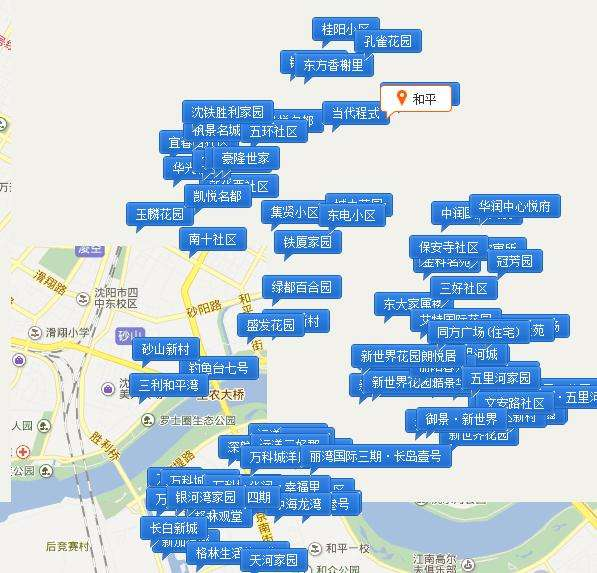
\includegraphics[scale=0.5]{jhtt}
\caption{某个点聚合图的实例}
\label{fig:jhtt}
\end{figure} \par
在拥有Mapbox和WebGL这两个强有力的工具后,我们还有两个最主要的任务需要解决:\par
\begin{itemize}
    \item {如何聚合?即给定一个点,以此为圆心,如何找到一定半径范围内所有点?}
    \item {聚合完毕后,给定一个包围盒(例如当前视口),如何找到其中包含的聚合后的要素?}
\end{itemize} \par
可以看出,对于这两个问题(radius \& range query),在海量点数据下,如果使用暴力遍历每个点的方法必然是低效的。为了高效搜索,我们需要上面介绍的K-D Tree。

\subsubsection{配合KNN算法实现数据分类}
KNN(K-Nearest Neighbor)算法,即K最近邻算法。\par
K最近邻,就是K个最近的相邻的元素的意思,说的就是每个样本都可以用距离它最近的K个邻居来代表。核心思想是如果一个样本在一定的空间中中的K个最相似或者最相近的样本中的大多数被标记为某一类,则该样本也会被标记为这一类,并具有这个类别上样本的特性。
\newpage
\begin{figure}[h!]
    \centering
    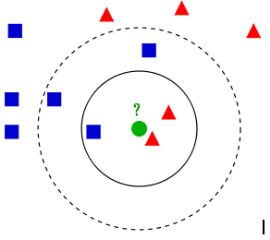
\includegraphics[scale=0.5]{KNN}
    \caption{KNN算法的模型}
    \label{fig:KNN}
\end{figure} \par
在使用KNN算法进行分类时,对某个新给定的样本,根据其k个距离最近的训练样本的类别,通过数量和距离权重分别计算的方式进行预测。由于KNN模型的空间一般是n维实数向量,所以通常用欧几里得距离来表示样本间的距离。该算法的关键是选取合适的k值,如果k值太小就意味着整体模型变得复杂,容易发生过拟合,即如果邻近的实例点恰巧是干扰项、噪声,预测的结果就会出现问题,极端的情况是k=1,称为最近邻算法,对于待预测点x,与x最近的点决定了x的类别。k值太大意味着整体的模型过于简单,极端的情况是k=N,那么无论新给定的样本是什么,都直接预测它属于训练集中最多的类,这样的模型显然不够严谨。\par
实现k近邻法时,主要考虑的问题是如何对训练数据进行快速k近邻搜索,这直接影响了这个算法的效率,是整个算法的核心所在。\par
而求相邻K个最近元素则是K-D Tree的用处之一,加之其运行效率较高,即可以配合KNN算法解决数据分类问题。

\subsubsection{配合SIFT算法实现图像匹配}
尺度不变特征转换(Scale-invariant feature transform或SIFT)是一种电脑视觉的算法用来侦测与描述影像中的局部性特征,它在空间尺度中寻找极值点,并提取出其位置、尺度、旋转不变量,此算法由 David Lowe在1999年所发表,2004年完善总结。\par
其应用范围包含物体辨识、机器人地图感知与导航、影像缝合、3D模型建立、手势辨识、影像追踪和动作比对。\cite{ref8}\par
此算法有其专利,专利拥有者为英属哥伦比亚大学。\par
局部影像特征的描述与侦测可以帮助辨识物体,SIFT 特征是基于物体上的一些局部外观的兴趣点而与影像的大小和旋转无关。对于光线、噪声、些微视角改变的容忍度也相当高。基于这些特性,它们是高度显著而且相对容易撷取,在母数庞大的特征数据库中,很容易辨识物体而且鲜有误认。使用 SIFT特征描述对于部分物体遮蔽的侦测率也相当高,甚至只需要3个以上的SIFT物体特征就足以计算出位置与方位。在现今的电脑硬件速度下和小型的特征数据库条件下,辨识速度可接近即时运算。SIFT特征的信息量大,适合在海量数据库中快速准确匹配。\cite{ref9}\par
SIFT算法的实质是在不同的尺度空间上查找关键点(特征点),并计算出关键点的方向。SIFT所查找到的关键点是一些十分突出,不会因光照,仿射变换和噪音等因素而变化的点,如角点、边缘点、暗区的亮点及亮区的暗点等。\cite{ref9}\par
SIFT的特点如下\cite{ref10}:\par
\begin{enumerate}
    \item {SIFT特征是图像的局部特征,其对旋转、尺度缩放、亮度变化保持不变性,对视角变化、仿射变换、噪声也保持一定程度的稳定性;}
    \item {独特性好,信息量丰富,适用于在海量特征数据库中进行快速、准确的匹配;}
    \item {多量性,即使少数的几个物体也可以产生大量的SIFT特征向量;}
    \item {高速性,经优化的SIFT匹配算法甚至可以达到实时的要求;}
    \item {可扩展性,可以很方便的与其他形式的特征向量进行联合。}
\end{enumerate} \par
当SIFT算法计算出图像的特征点(特征向量)之后,只需要在高维空间中查询相距最近的若干特征向量组便可实现图像匹配。\par
显然,上述操作可以使用K-D Tree实现。

\section{总结}
总的来说,这学期的计算科学导论使我受益良多。在孙老师的课堂上,我不仅仅接触到了科学哲学与哲学方法论,还接触了令人神往的一系列计算科学知识,例如计算的数学理论,在孙老师的指引和鼓励下,我学会了搜索、阅读期刊,并且由课内知识向外延伸,接触了确定性有限状态自动机理论,并且接触了强大而优美的用于处理字符串匹配问题的数据结构——后缀自动机。\par
在孙老师精心设计的分组演讲环节中,我与我的搭档赵成齐心协力,不仅提升了个人能力,还锻炼了团队合作的能力与精神,并且了解了广泛应用于生产生活的数据结构——K-D Tree。\par
孙老师常常教导我们要做爱国爱党、符合社会主义核心价值观的计算机科学与技术专业人才。无论做什么,都要坚守本心,恪守作为一个中国公民的道德准则。在孙老师的熏陶下,我下定决心,要用奋斗和青春为祖国的计算机科学事业增光添彩。

\newpage

\section{附录}
\begin{itemize}
    \item {
        \bf{Github}\\
        Profile: https://github.com/Sulfur6\\
        Github Page: https://sulfur6.github.io/
        \begin{figure}[h]
            \centering
            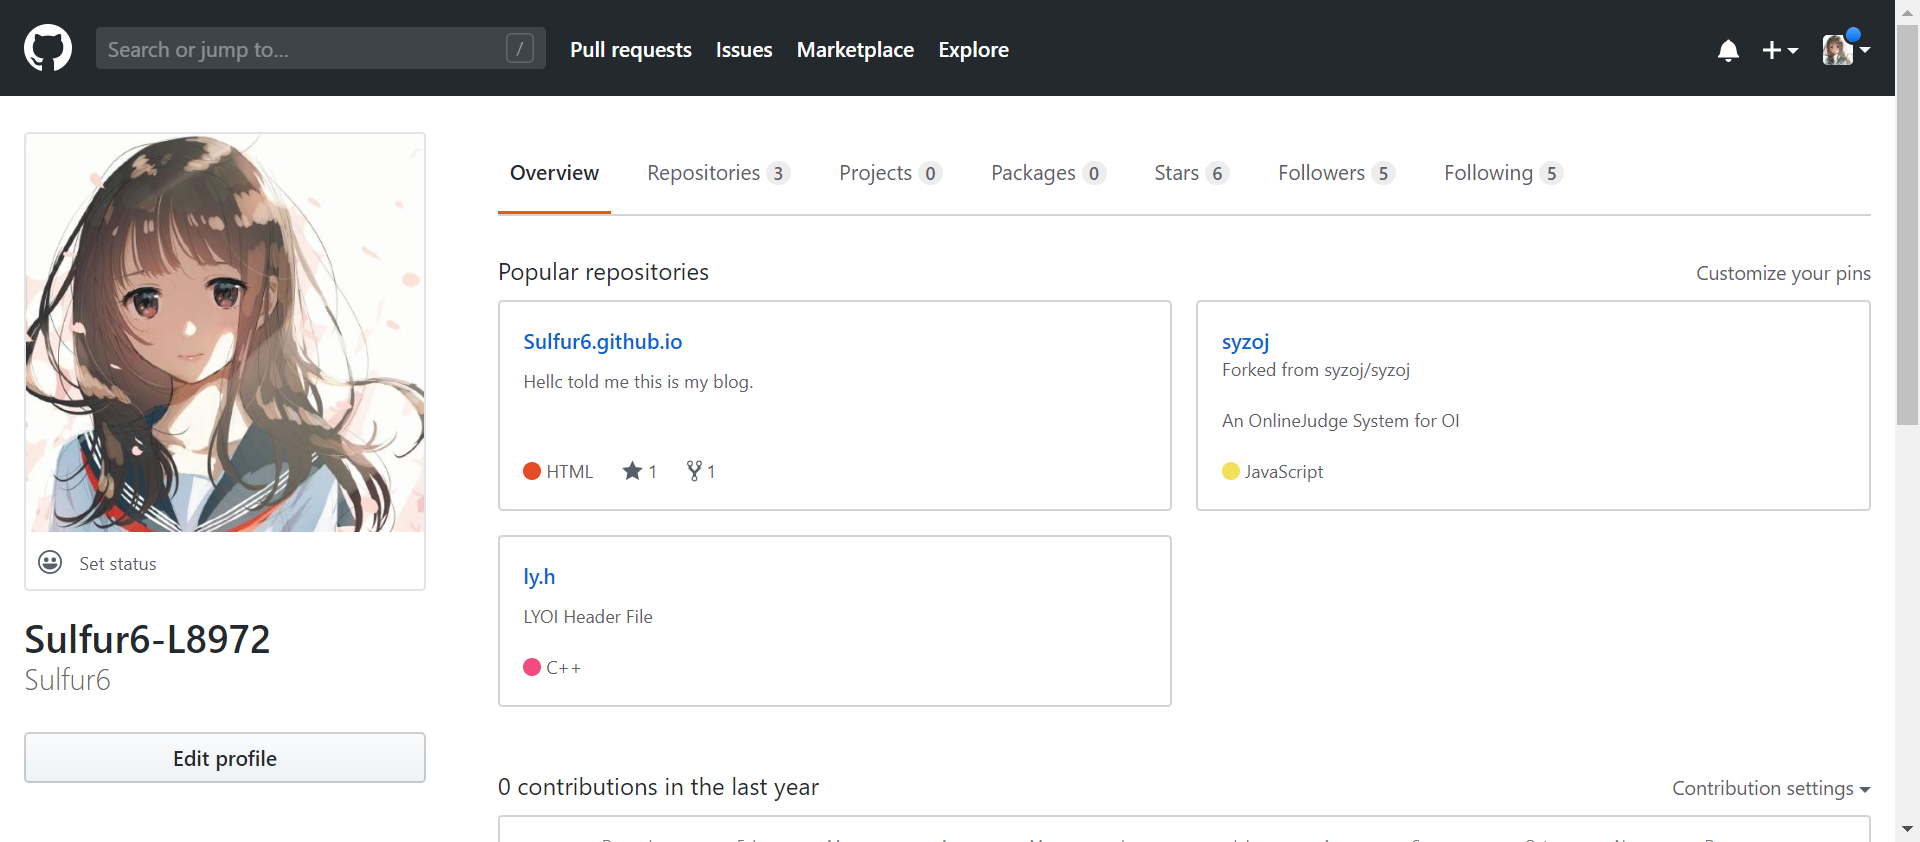
\includegraphics[scale=0.4]{github}
            \label{fig:github}
        \end{figure}
    }
\newpage
    \item {
        \bf{观察者网}\\
        \begin{figure}[h]
            \centering
            
\includegraphics[scale=0.1]{gcz}
            \label{fig:gcz}
        \end{figure}
    }
    \item {
        \bf{学习强国}\\
        \begin{figure}[h]
            \centering
            
\includegraphics[scale=0.1]{xxqg}
            \label{fig:xxqg}
        \end{figure}
    }
\newpage
    \item {
        \bf{哔哩哔哩}\\
        \begin{figure}[h]
            \centering
            
\includegraphics[scale=0.1]{bilibili}
            \label{fig:bilibili}
        \end{figure} 
    }
    \item {
        \bf{CSDN}\\
        CSDN Blog: https://blog.csdn.net/Sulfur6\\
        \begin{figure}[h]
            \centering
            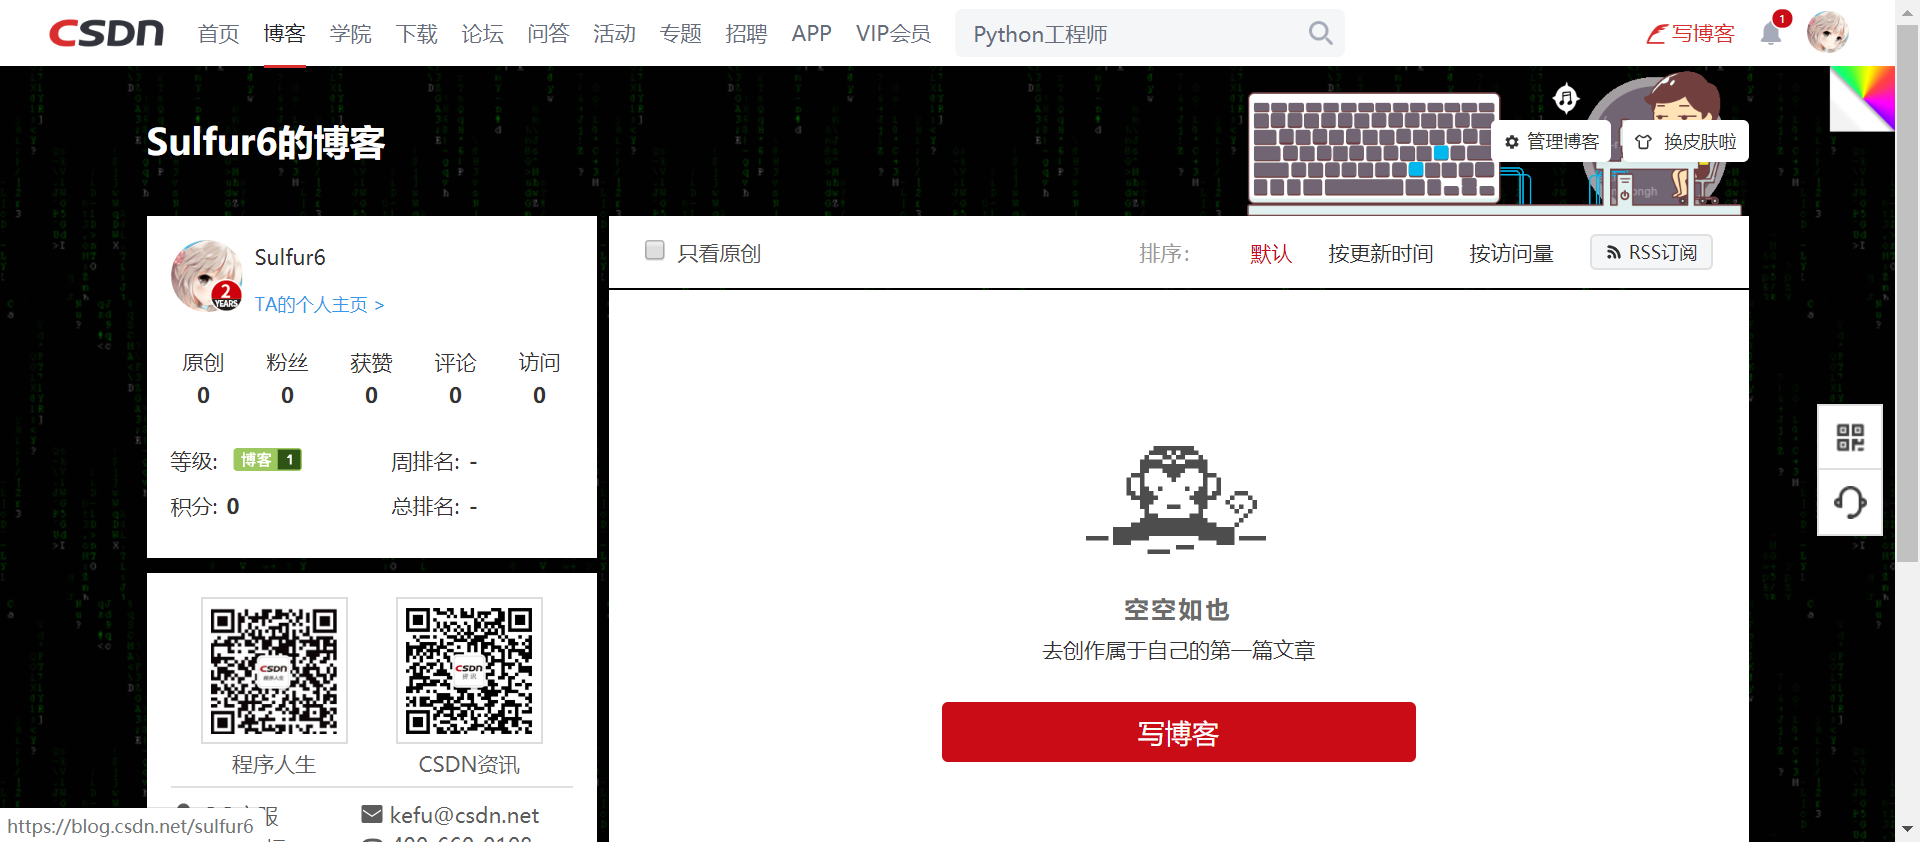
\includegraphics[scale=0.4]{csdn}
            \label{fig:csdn}
        \end{figure}
    }
    \item {
        \bf{博客园}\\
        https://www.cnblogs.com/Sulfur6/\\
        \begin{figure}[h]
            \centering
            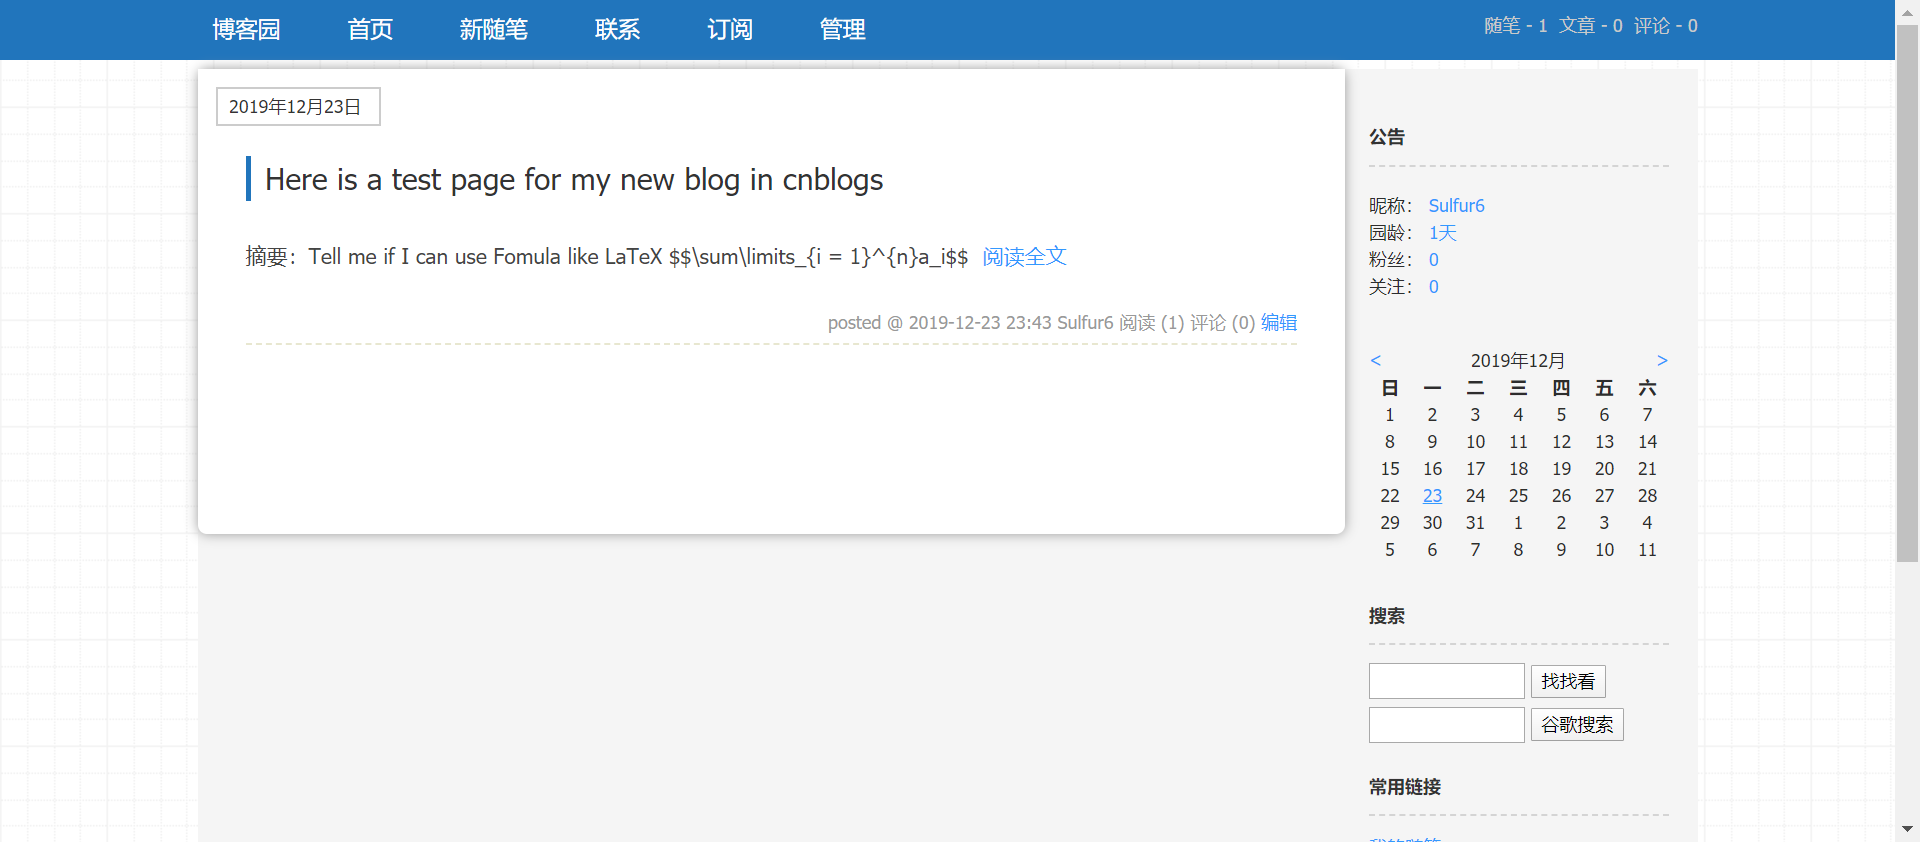
\includegraphics[scale=0.4]{cnblogs}
            \label{fig:cnblogs}
        \end{figure} 
    }
\newpage
    \item {
        \bf{小木虫}\\
        http://muchong.com/bbs/space.php?uid=20248196\\
        \begin{figure}[h]
            \centering
            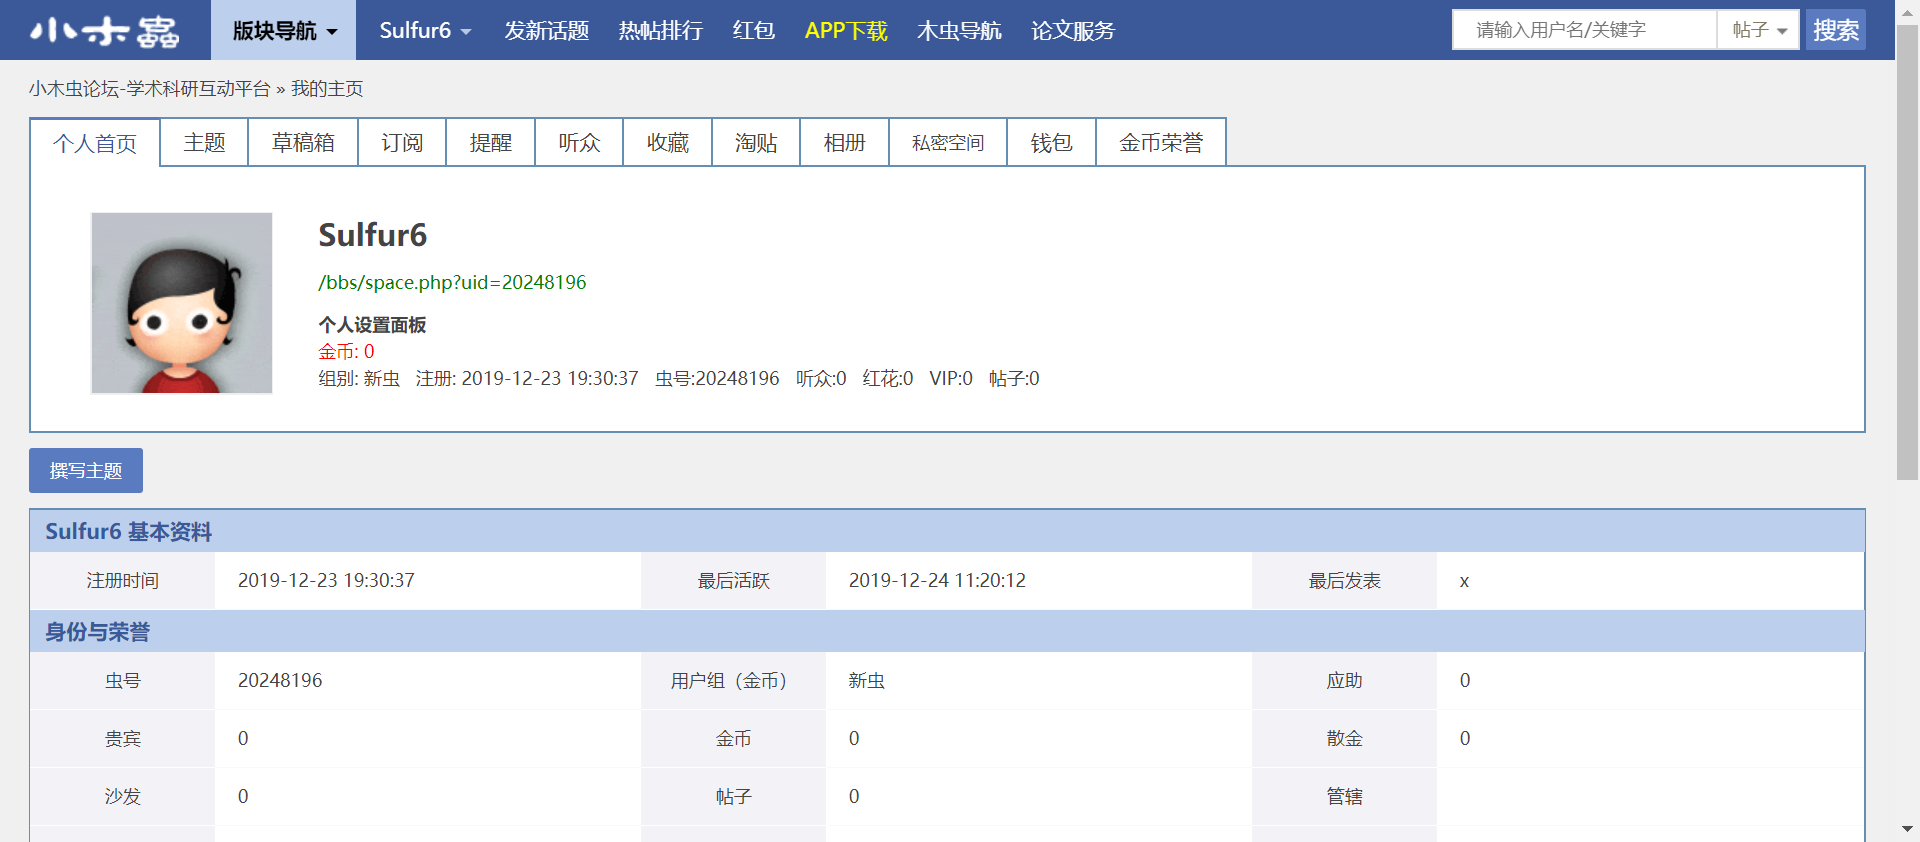
\includegraphics[scale=0.4]{xmc}
            \label{fig:xmc}
        \end{figure}  
    }
\end{itemize}

\newpage

\bibliographystyle{plain}
\bibliography{references}
\begin{thebibliography}{99}  
    \bibitem{ref1}Hopcroft, John E.; Motwani, Rajeev; Ullman, Jeffrey D. (2001). Introduction to Automata Theory, Languages, and Computation (2 ed.). Addison Wesley. ISBN 0-201-44124-1. Retrieved 19 November 2012.
    \bibitem{ref2}Lawson, Mark V. (2004). Finite automata. Chapman and Hall/CRC. ISBN 1-58488-255-7. Zbl 1086.68074
    \bibitem{ref3}Michael Sipser, Introduction to the Theory of Computation. PWS, Boston. 1997. ISBN 0-534-94728-X.
    \bibitem{ref4}Blumer, A.; Blumer, J.; Haussler, D. (1985), "The smallest automation recognizing the subwords of a text.", Theoretical Computer Science, 40: 31–55, doi:10.1016/0304-3975(85)90157-4
    \bibitem{ref5}Brown RA (2015). "Building a balanced k-d tree in O(kn log n) time". Journal of Computer Graphics Techniques. 4 (1): 50–68.
    \bibitem{ref6}Freidman, J. H.; Bentley, J. L.; Finkel, R. A. (1977). "An Algorithm for Finding Best Matches in Logarithmic Expected Time". ACM Transactions on Mathematical Software. 3 (3): 209. doi:10.1145/355744.355745
    \bibitem{ref7}Lee, D. T.; Wong, C. K. (1977). "Worst-case analysis for region and partial region searches in multidimensional binary search trees and balanced quad trees". Acta Informatica. 9. doi:10.1007/BF00263763
    \bibitem{ref8}Lowe, David G. (1999). "Object recognition from local scale-invariant features". Proceedings of the International Conference on Computer Vision. 2. pp. 1150–1157. doi:10.1109/ICCV.1999.790410
    \bibitem{ref9}U.S. Patent 6,711,293, "Method and apparatus for identifying scale invariant features in an image and use of same for locating an object in an image", David Lowe's patent for the SIFT algorithm, March 23, 2004
    \bibitem{ref10}Lowe, David G. (2004). "Distinctive Image Features from Scale-Invariant Keypoints". International Journal of Computer Vision. 60 (2): 91–110. CiteSeerX 10.1.1.73.2924. doi:10.1023/B:VISI.0000029664.99615.94
\end{thebibliography}


\end{document}
